\chapter{Basic Analysis \& Corrections}

\section{Introduction}
Several analysis components are common to both main analyses presented in this thesis.  During this chapter, I discuss the calculation of luminosity, vertex corrections, timing corrections, and kinematic corrections.  

\section{Luminosity Calculation}
A useful concept in accelerator/collider physics is the luminosity $\mathcal{L}$.  Luminosity is defined as the number of collisions per unit area per unit time that could lead to some process of interest.  Consider as an example elastic scattering of electrons from protons, the luminosity is the number of electron-proton collisions per unit time per unit area.  The rate $\frac{dN}{dt}$ of the occurance of events for some process $X$ can be written in terms of this luminosity and the cross section for the process.

\begin{equation}
	\frac{dN_X}{dt} = \mathcal{L} \sigma_X 
\end{equation}

For the fixed target case, the luminosity has a simple expression.

\begin{equation}
	\mathcal{L} = \frac{j_e \rho_p l_T}{e} 
\end{equation}

Here $l_t$ is the target length, $\rho_p$ is the proton number density in the target, and $j_e$ is the beam current. To find the total number of events which accumulate in some time $t_{exp}$ the event rate is integrated with respect to time.

\begin{align}
	N_X = \int_{0}^{t_{exp}} \frac{j_e \rho_p l_T}{e} \sigma_X dt \\
	= \frac{\rho_p l_T}{e} \sigma_X \int_{0}^{t_{exp}} j_e dt \\
	=  \frac{\rho_p l_T}{e} \sigma_X \Delta Q
\end{align}

Thus the experimentally observed cross section for some process $X$ is,

\begin{equation}
	\sigma_{X} = \frac{N_{X}}{\mathcal{L}_{int}}
\end{equation}

where the number of events $N_X$ is corrected for all effects and $\mathcal{L}_{int}$ is the integrated luminosity as shown above. \\

Experimentally, the factor $\Delta Q$ can be calculated from charge deposition measurements by the Faraday cup.  The Faraday cup charge is a scalar value written periodically into the output event stream, not with every recorded event.  This information is stored in the output BOS files in a bank called \texttt{TRGS}, the variable is named \texttt{FCUP\_G2}.  \\

For this data analysis, the final ntuple (root files) used did not contain the Faraday cup charge information.  For this reason, the authors used the BOS files directly and recorded the value of \texttt{FCUP\_G2} for every scalar reading, as well as the event number directly after each scalar entry (from the \texttt{HEAD} bank).  This event number correlates directly to the event number stored in the root files used for analysis. \\

The total accumulated charge over a run is simply the sum over consecutive differences in the Faraday cup charge.

\begin{equation}
	\Delta Q = \sum_{i=1}^{n-1} q[i+1]-q[i] 	
\end{equation}

Here $n$ denotes the number of scalar entries for a given file.  Due to the periodic nature of the scalar bank writing events are also recorded after the last reading of the file, and before the first scalar reading of the next file in the run.  To account for this the difference between consecutive files last and first readings is added to the total. \\

\easyFigure{image/plots/basic-analysis/entries.png}{Entries per scalar reading for run 38222.}
\easyFigure{image/plots/basic-analysis/charge.png}{Charge per scalar reading for run 38222.}

For the E1-F dataset, a run typically contains around 20 files, each representing a raw file size of 2 gigabytes.  These files are named by run number, and given an index from $0$ to $n_{files}-1$.  It is not uncommon that a run will contain missing files in the middle of the range.  If this occurs, the charge difference between last/first reading is not added to the total. \\

Any charge which accumulates in a period of time where the number of events did not change is not added to the total.  Similarly, any events which occur within regions where no charge is recorded need to be discarded.  This is accomplished by recording the bad event ranges for every file and removing these events from our analysis. \\

The result of this procedure is a numerical value of charge for each run.  For practitioners, it is important to note that this value needs to be scaled by the DAQ scaling factor before it represents a value of charge.  In our analysis, the numerical value of charge for a typical file is a few tens of micro-Coulombs.

\section{Determination of Good Run List}
The total dataset contains 831 runs.  Due to the complexities of the CLAS experimental setup, it is not uncommon for run conditions to change between runs such that a portion of the data collected are not of analysis quality.  For this reason, a good run list is constructed. \\

Good runs are selected for the list by counting good electrons in each file and normalizing by the accumulated charge for the associated file.  For each file, the difference between subsequent Faraday cup readings is summed to calculate the charge for the file.  Creation of the total charge for the run includes an additional contribution from endpoints in adjacent files.  This extra charge builds up after the last scalar reading of one file and before the first scalar bank in the new adjacent file.  While the number of events collected varies from run to run the ratio defined above is a stable quantity -- provided that the run conditions do not vary greatly.  Good runs were chosen to have $N/Q > 4000$ based on inspection of the figure \ref{fig:inclusive_rates}.  

\begin{figure}
	\label{fig:inclusive_rates}
	\begin{center}
		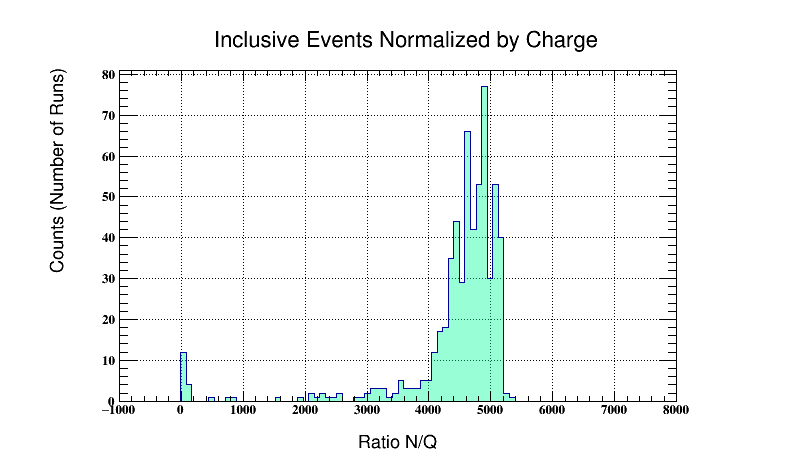
\includegraphics[width=14cm]{image/plots/basic-analysis/inclusive-rates.png}
		\caption{Inclusive electrons per file normalized by the total charge accumulated for the file.  This quantity is used to make a good run list.}
	\end{center}
\end{figure}

\section{Helicity Determination}
During the course of the E1-F run period the beam helicity convention was changed by the insertion of a half-wave plate at the injector.  The definition of $\pm$ helicity must change in accordance with these wave-plate insertions.  To monitor these changes, the value of $A_{LU}^{\sin\phi}$ for $\pi^+$ is recorded for every run.  Whenever the asymmetry (which has a magnitude of around $3\%$) changes sign, the sign convention has changed.  These changes are taken into account in the data analysis.   

\easyFigure{image/plots/basic-analysis/bsa-waveplate.pdf}{The waveplate position is determined and corrected by plotting the BSA for $\pi^{+}$ mesons as a function of the run.  The top panel shows the corrected results, the bottom shows the results before changing the helicity.}

\section{Vertex Corrections}
The track vertex position $(v_x, v_y, v_z)$ is calculated based on the intersection of each track with the midplane (the plane which contains the beamline and bisects the sector at $\phi_{rel} = 0$).  If the beam is not centered at $(x,y)=(0,0)$, the vertex position calculation needs to be corrected by shifting the midplanes in accordance with the target offset.  The offset $(x,y)$ is identified by plotting events from the control foil placed near the target, which has a $z$ position of 20 cm. For the E1-F run period, the beam position was (0.15, -0.25) cm.  This correction is applied to the entire data set based on this position, and its successful effect is shown in figure \ref{fig:vertex_phi}.  In practice the beam position may vary more frequently than in our case, and the correction would be applied run-by-run, here it is not necessary.  \\

\begin{figure}
	\label{fig:vertex_phi}
	\begin{center}
		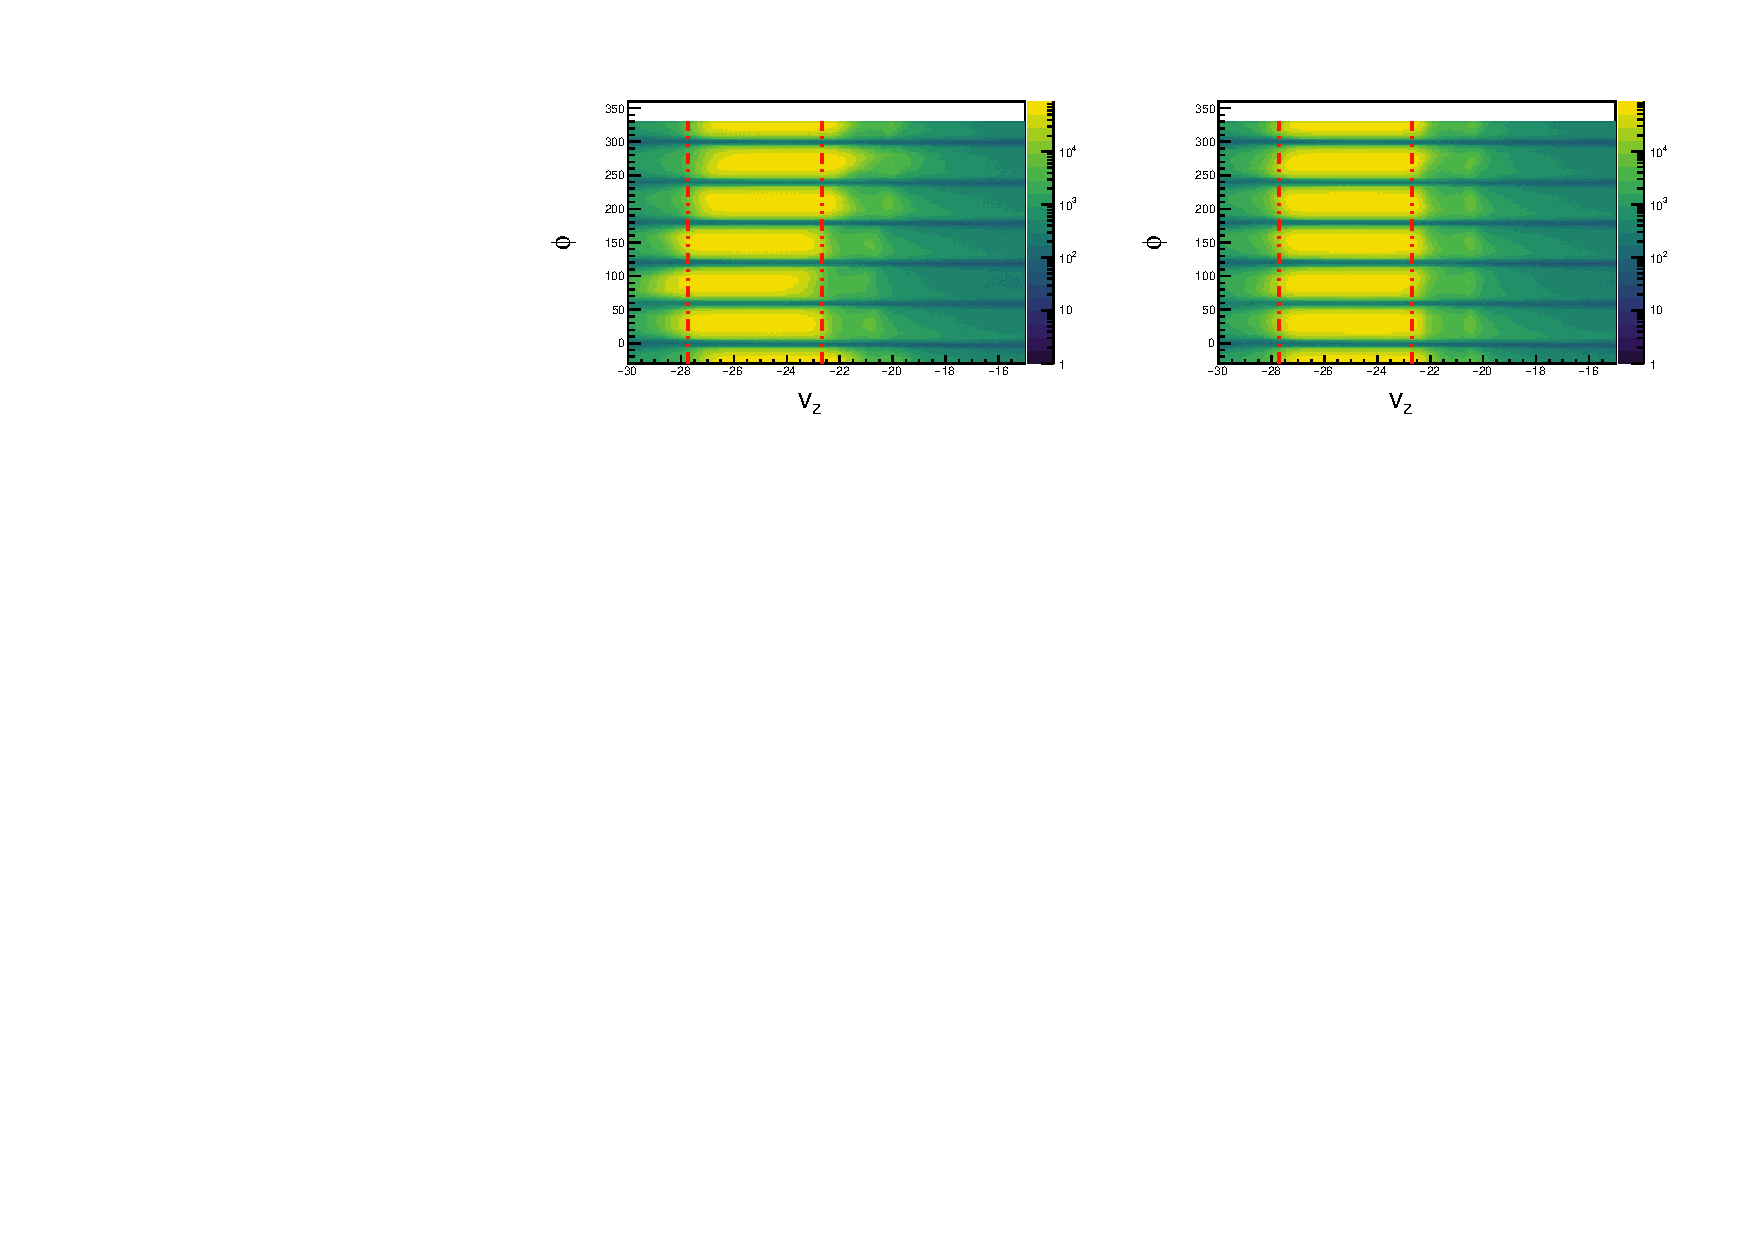
\includegraphics[width=14cm]{image/plots/basic-analysis/vertex-phi.pdf}
		\caption{The z-vertex $v_z$ position shown for different values of $\phi$ the azimuthal angle in the hall.  The left figure shows the distribution before corrections are applied, the right after.  The vertical red lines bound the region which we define as acceptable for electrons in our analysis.}
	\end{center}
\end{figure}

\section{Timing Corrections}
Timing information comes from the time-of-flight detector system.  After calibration, small offsets in timing between time of flights paddles still exist for the E1-F dataset.  These biases can be removed on a run-by-run and paddle-by-paddle basis by adding a small shift $t_{corr}$.  In order to determine this shift $t_{corr}$ for each paddle, charged pions are used.  \\

Using momentum from the drift chambers the value of $\beta$ can be predicted and the difference $\Delta \beta$ can be determined for each pion. 

\begin{equation}
	\Delta \beta = \beta_{obs} - \beta_{pred} = \frac{d}{c t_{obs}} - \sqrt{1+(m/p)^2} 
\end{equation} 

Here m is assumed to be $m_{\pi}$.  The offset $\Delta \beta$ from 0 is used to define the value of $t_{corr}$ for each paddle.  If this value is exceedingly small, no correction is applied.  For some paddles with low statistics a reasonable value for $t_{corr}$ cannot be obtained and these paddles are excluded from the analysis.  \\

\easyFigure{image/plots/basic-analysis/timing.pdf}{Timing corrections are shown for paddle 24 of sector 1.  The left image shows the $\Delta \beta$ distribution before corrections.  On the right the same is shown after correction of the timing for this paddle.  We assume the mass of the track to be the pion, these show up as the green band.  Heavier protons are visible below the pion band.}

In the method described above, the calibrated paddle is the one which is struck by the pion.  The electron paddle which was struck could also require calibration.  In practice the magnitude of the correction term $t_{corr}$ is small, and the paddle offset is (likely) randomly distributed about 0 when considering all paddles.  By including events from many different (electron) paddles, miscalibration effects from the electron side cease to be important.  This is demonstrated by the success of the technique in centering the $\Delta \beta$ distributions.  This work was first described in \cite{theses-harrison:2015}. \\

\section{Kinematic Corrections}
The magnetic field map used in reconstruction to swim particle tracks cannot perfectly match the real magnetic field of the hall.  As a result of this the reconstructed momentum of particles is often slightly off (of order 1\%).  Small misalighments in detector positions also contribute to this effect.  In order to correct for these small differences, the momentum $(p_x, p_y, p_z)$ and hence $\theta$ of charged tracks is corrected. \\

Various proceedures exist for the correction of kinematic variables of measured particles, and they all rely on energy and momentum conservation applied to standard processes (such as elastic scattering).  The procedure used to derive corrections for the E1-F dataset was developed and described by Marco Mirazita in \cite{misc-mirazita:2010}.  \\

As mentioned previously, the need for correction to $\theta$ (the polar angle measured from the beamline) arises from misalignments in the drift chambers.  This implies that the correction will be the same for positives and negatives, and this assumption is used in the correction algorithm.  First, elastic $(ep \rightarrow ep)$ events are selected by identifying events that contain at least one electron and one proton, then requiring that the missing mass $M_X$ of the ($ep \rightarrow epX$) system is close to 0.  The kinematics of the event are then calculated.

\begin{gather}
	k^{\mu} = (k, 0, 0, k)                         \\
	p^{\mu} = (M_{p}, 0, 0, 0)                     \\
	k'^{\mu} = (k', k'\sin\theta, 0, k'\cos\theta) \\
	p'^{\mu} = (E_{p}, -p'\sin\alpha, 0, p'\cos\alpha) 
\end{gather}

Applying energy and momentum conservation to the equations above yields 3 equations.

\begin{gather}
	k + M_p = k' + \sqrt{M_{p}^{2} + p'^2} \\
	k'\sin\theta = p'\sin\alpha            \\
	k = k'\cos\theta + p'\cos\alpha  
\end{gather}

Using these equations, the electron angle $\theta$ and the proton angle $\alpha$ can be predicted by using the momenta $(k',p')$.  These values are compared with measured values and iteratively corrected by tuning the parameters of a phi-dependent 2nd order polynomial.

\begin{gather}
	\cos\theta = 1 - M_p \frac{k-k'}{kk'} \\
	\tan\alpha = \frac{1}{p'} \frac{k'\sin\theta}{k-k'\cos\theta}
\end{gather}

After $\theta$ corrections are applied, the momentum of the electrons are corrected by using an analogous procedure for $k'$ instead of $\theta$ and $\alpha$.  The momentum corrections are calculated as functions of $\phi$ for each sector in one degree bins of $\theta$.  Finally, the positively charged particles momenta are corrected by selecting the exclusive event $(ep \rightarrow e\pi^+N)$.  In this reaction the scattered electron and pion are detected and the neutron is selected using a missing mass cut.  Assuming the electron momentum, electron angle, and pion angle to be correct, the pion momentum correction is then calculated by iteratively improving the central position of the neutron mass peak to coincide with $M_{N}$.  Marco Mirazita shows in his note that these corrections can be satisfactorily applied to all negative and positive particles.

\easyFigure{image/plots/basic-analysis/phi-dw-uncorr.pdf}{This figure shows the deviation from $M_p$ of the $W$ spectrum peak for elastic $ep \rightarrow ep$ events (before corrections).}
\easyFigure{image/plots/basic-analysis/phi-dw-corr.pdf}{This figure shows the deviation from $M_p$ of the $W$ spectrum peak for elastic $ep \rightarrow ep$ events (after $\phi$-dependent corrections).}
\easyFigure{image/plots/basic-analysis/w-mom-corr.png}{Elastic events shown in the spectrum of $W$ before and after momentum corrections are applied.}
